\begin{figure}[h!]
\centering
\resizebox{\linewidth}{!}{%
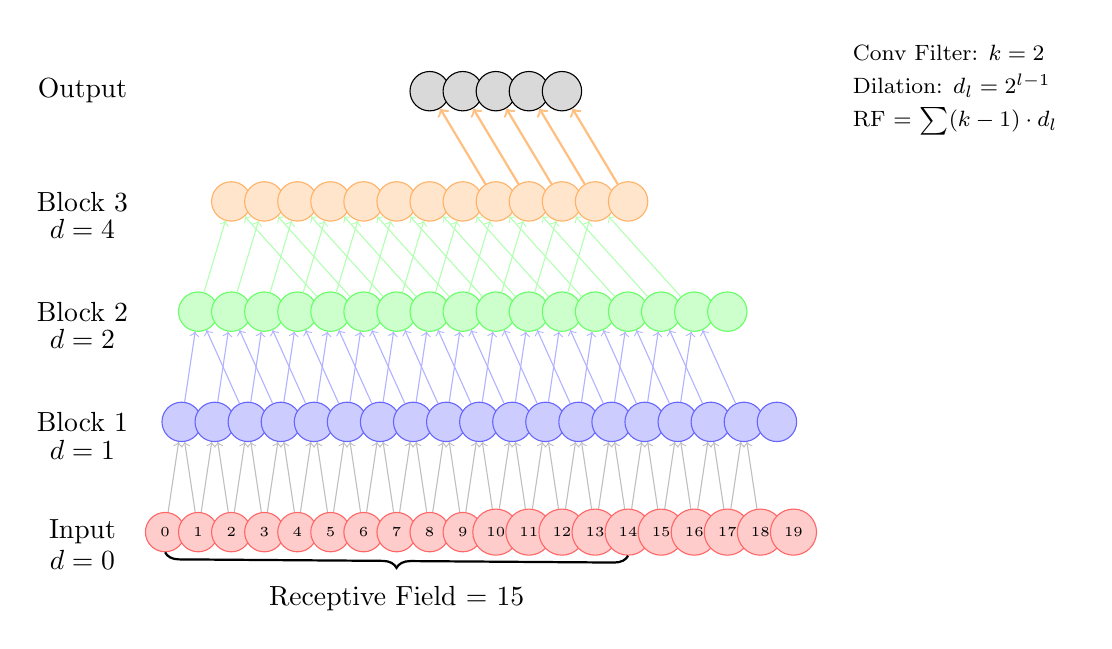
\begin{tikzpicture}[scale=0.7]
    % Define styles
    \tikzstyle{input} = [circle, draw=red!60, fill=red!20, minimum size=0.5cm]
    \tikzstyle{hidden1} = [circle, draw=blue!60, fill=blue!20, minimum size=0.5cm]
    \tikzstyle{hidden2} = [circle, draw=green!60, fill=green!20, minimum size=0.5cm]
    \tikzstyle{hidden3} = [circle, draw=orange!60, fill=orange!20, minimum size=0.5cm]
    \tikzstyle{output} = [circle, draw=black, fill=gray!30, minimum size=0.5cm]
    
    % Input layer (t=0 to t=19 for window size 20)
    \foreach \x in {0,...,19} {
        \node[input] (i\x) at (\x*0.6, 0) {\tiny\x};
    }
    \node at (-1.5, 0) {Input};
    \node at (-1.5, -0.5) {$d=0$};
    
    % Hidden layer 1 (d=1)
    \foreach \x in {0,...,18} {
        \node[hidden1] (h1\x) at (\x*0.6 + 0.3, 2) {};
    }
    \node at (-1.5, 2) {Block 1};
    \node at (-1.5, 1.5) {$d=1$};
    
    % Hidden layer 2 (d=2)
    \foreach \x in {0,...,16} {
        \node[hidden2] (h2\x) at (\x*0.6 + 0.6, 4) {};
    }
    \node at (-1.5, 4) {Block 2};
    \node at (-1.5, 3.5) {$d=2$};
    
    % Hidden layer 3 (d=4)
    \foreach \x in {0,...,12} {
        \node[hidden3] (h3\x) at (\x*0.6 + 1.2, 6) {};
    }
    \node at (-1.5, 6) {Block 3};
    \node at (-1.5, 5.5) {$d=4$};
    
    % Output layer
    \foreach \x in {0,...,4} {
        \node[output] (o\x) at (\x*0.6 + 4.8, 8) {};
    }
    \node at (-1.5, 8) {Output};
    
    % Connections for d=1 (kernel size=2)
    \foreach \x in {0,...,17} {
        \pgfmathtruncatemacro{\next}{\x+1}
        \draw[gray!50, ->] (i\x) -- (h1\x);
        \draw[gray!50, ->] (i\next) -- (h1\x);
    }
    
    % Connections for d=2
    \foreach \x in {0,...,15} {
        \pgfmathtruncatemacro{\next}{\x+1}
        \pgfmathtruncatemacro{\skip}{\x+2}
        \draw[blue!30, ->] (h1\x) -- (h2\x);
        \draw[blue!30, ->] (h1\skip) -- (h2\x);
    }
    
    % Connections for d=4
    \foreach \x in {0,...,11} {
        \pgfmathtruncatemacro{\skip}{\x+4}
        \draw[green!30, ->] (h2\x) -- (h3\x);
        \draw[green!30, ->] (h2\skip) -- (h3\x);
    }
    
    % Output connections
    \foreach \x in {0,...,4} {
        \pgfmathtruncatemacro{\idx}{\x+8}
        \draw[orange!50, thick, ->] (h3\idx) -- (o\x);
    }
    
    % Receptive field visualization
    \draw[decorate, decoration={brace, amplitude=5pt, mirror}, thick] 
        (i0.south) -- (i14.south) node[midway, below=8pt] {Receptive Field = 15};
    
    % Annotations
    \node[above right] at (12, 7) {
        \begin{tabular}{l}
        \footnotesize Conv Filter: $k=2$ \\
        \footnotesize Dilation: $d_l = 2^{l-1}$ \\
        \footnotesize RF = $\sum (k-1) \cdot d_l$
        \end{tabular}
    };
    
\end{tikzpicture}
}

\caption{Dilated Causal Convolution with Exponentially Increasing Receptive Field}
\label{dif:dilated_conv}
\end{figure}